\chapter{Mission} % <<< ---------------------------------------------------------------------------------
\label{ch:mission}
% ---------------------------------------------------------------------------- %

This chapter  presents a brief overview  of the hardware platform  and some of
its key  characteristics which are  of interest to us. From  that information,
the objectives of this project are derived. Possible approaches to reach those
objectives are  presented and evaluated, and  a decision is reached  on how to
achieve this project's aims.


\section{The Red Pitaya STEMlab 125-14} % <<< -------------------------------- %
\label{sec:stl125}
% ---------------------------------------------------------------------------- %

The  device on  which this  project  is based  is the  Pitaya STEMlab  125-14,
pictured  in Figure~\ref{fig:stl125:photo}. STEMlab  is a  compact measurement
instrument (fits  into the palm  of a hand)  which can replace  more expensive
devices like  oscilloscopes by using  a computer for data  storage, processing
and presentation.

Some of its key specifications relavant to us are:
\begin{itemize}\tightlist
    \item
        two analog inputs and outputs via coaxial connectors
    \item
        resolution of ADC for those inputs: \num{14}\,bits per channel
    \item
        ADC sampling rate: \num{125}\,MS$\cdot$s\textsuperscript{-1}
    \item
        Xylinx SOC  with an FPGA component  for data processing on  the device
        itself and two ARM Cortex9 chips for general-purpose tasks
    \item
        Ethernet  connection and  USB  connections for  data transmission  and
        device control
    \item
        Has its own operating system, a GNU/Linux distribution (Ubuntu is used
        in our project), running on the ARM cores.
    \item
        The software used is open-source and available under \cite{pita:github}.
\end{itemize}
More  comprehensive documentation  can be  found at~\cite{pita:readthedocs}. A
block   diagram   with    the   system's   key   components    is   shown   in
Figure~\ref{fig:stl125:block_diagram}.

\cite{bucher:kuery}

Input voltage rating, ADC spec sheet, \ldots

\begin{figure}
    \centering
    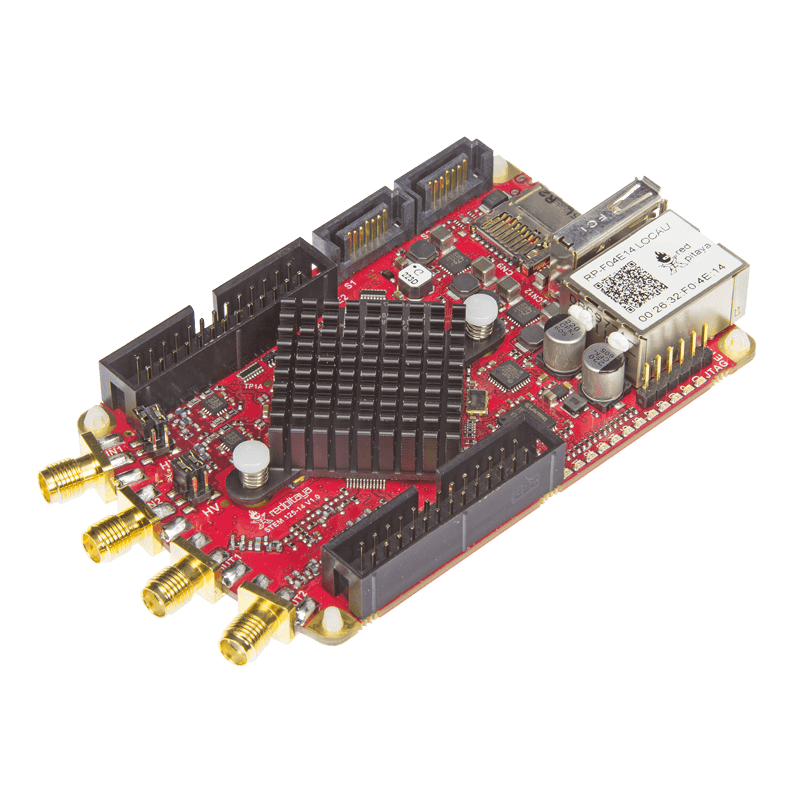
\includegraphics[width=0.67\textwidth]{images/stl125/stemlab125-14-photo.png}
    \caption{Block diagram of the Red Pitaya STEMlab. Source:~\cite{pita:elektor:starterkit}}
    \label{fig:stl125:photo}
\end{figure}

\begin{figure}
    \centering
    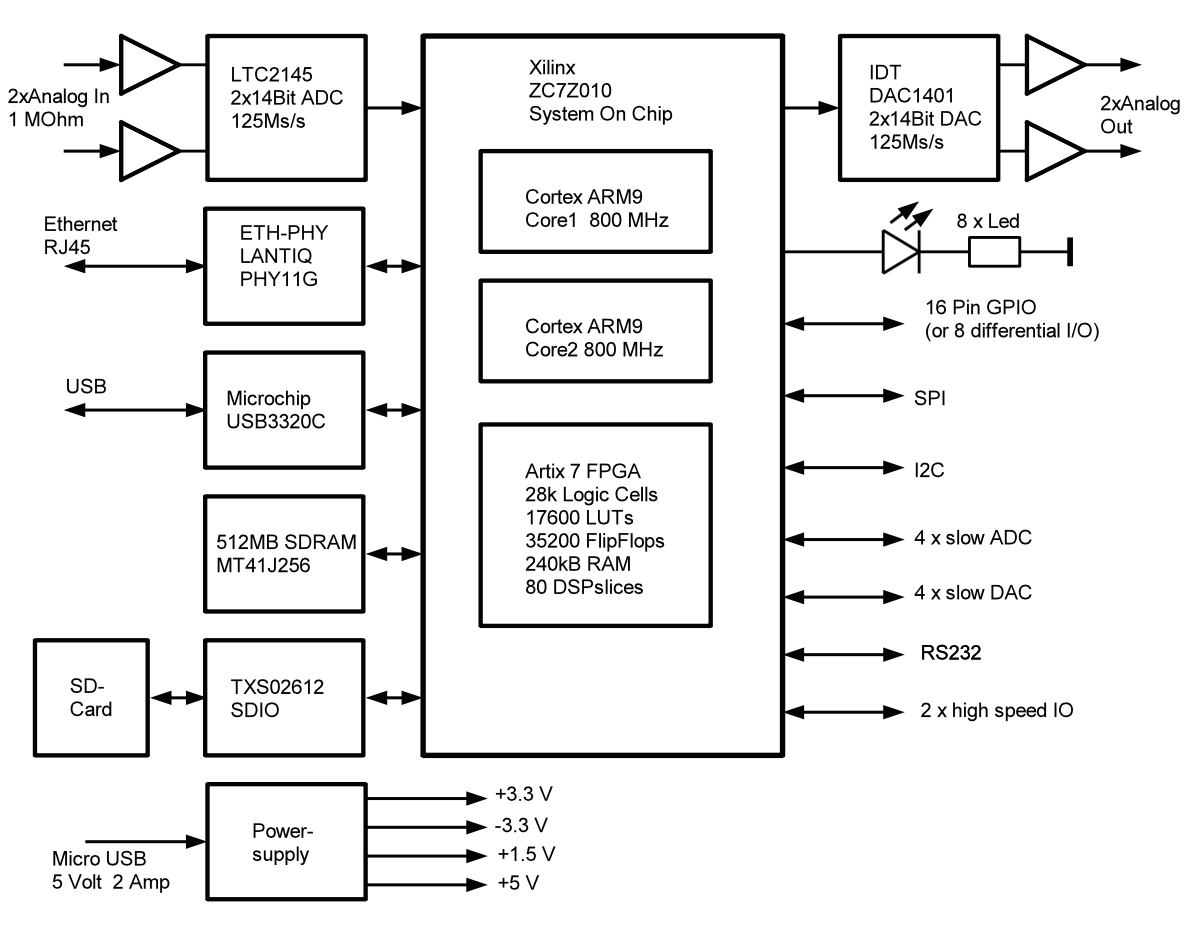
\includegraphics[width=\textwidth]{images/stl125/stemlab125.png}
    \caption{Block diagram of the Red Pitaya STEMlab. Source:~\cite{pita:ossmann}}
    \label{fig:stl125:block_diagram}
\end{figure}

%>>>

\begin{itemize}
    \item
        Initial situation
    \item
        decision process, possible solutions, decision matrix
        \begin{itemize}
            \item
                problems with orignal code base
            \item
                choice of own implementation
            \item
                choose own implementation based on Pavel's stuff
        \end{itemize}
    \item
        concept for solution
        \begin{itemize}
            \item
                Pavel's base
            \item
                use logger core
            \item
                write own server
            \item
                write own front-end
            \item
                use xilinx filter blocks where possible
        \end{itemize}
\end{itemize}


% >>>
%^^A vim: foldenable foldcolumn=4 foldmethod=marker foldmarker=<<<,>>>
